%%% The main file. It contains definitions of basic parameters and includes all other parts.


%% Settings for two-sided (duplex) printing
\documentclass[10pt,a4paper]{report}
\let\openright=\cleardoublepage

%% Character encoding: usually latin2, cp1250 or utf8:
\usepackage[utf8]{inputenc}

%% It's 2019
\usepackage[default]{droidserif}
\usepackage[T1]{fontenc}

%% Further useful packages (included in most LaTeX distributions)
\usepackage{amsmath}        % extensions for typesetting of math
\usepackage{amsfonts}       % math fonts
\usepackage{graphicx}       % embedding of pictures
\usepackage{tikz}
%\usetikzlibrary{shapes,fit,positioning,snakes,mindmap,trees,decorations.text,arrows.meta}
%\makenomenclature
\usepackage{algorithm,algpseudocode}
\usepackage{booktabs}
\usepackage{mwe}
\usepackage{pgfgantt}
\usepackage{pdflscape}
\usepackage{geometry}
\usepackage{enumitem}
\usepackage{float}
\usepackage{framed}
\usepackage{titlesec}
\usepackage{listings}
\usepackage{xcolor}
\usepackage{longtable}

\usepackage{multirow}

\lstset{basicstyle=\ttfamily,
	showstringspaces=false,
	commentstyle=\color{red},
	keywordstyle=\color{blue}
}

\usepackage{pdfpages}

\usepackage[textsize=tiny,backgroundcolor=yellow!50, linecolor=black!25]{todonotes}

% links shall be clickable
\usepackage[unicode]{hyperref}   % Must follow all other packages
\usepackage{cleveref} % Must follow all other packages including hyperref

% Definitions of macros (see description inside)

\newcommand{\cool}{\color{green!50!white!80!black}}
\newcommand{\textcool}[1]{{\cool #1}}

\newcommand{\XX}[1]{\textcolor{red}{#1}}
\newcommand{\TT}[1]{\texttt{#1}}
\newcommand{\SC}[1]{{\fontfamily{phv}\selectfont\textsc{#1}}}

% Draw black "slugs" whenever a line overflows, so that we can spot it easily.


% avoid some slugs naturally
\clubpenalty=1000
\widowpenalty=1000
%\hyphenpenalty=100  % turn this on to prevent hyphenation
\emergencystretch=2cm


%%% The field of all real and natural numbers
\newcommand{\R}{\mathbb{R}}
\newcommand{\N}{\mathbb{N}}
\newcommand{\F}{\mathbb{F}}
\newcommand{\Z}{\mathbb{Z}}

\newcommand{\bms}{\begin{enumerate}[label=\bf (M\arabic*)]}
\newcommand{\bwp}{\begin{enumerate}[label=\bf \normalsize  (WP\arabic*), resume=del]}
\newcommand{\eenum}{\end{enumerate}}
\newcommand{\itemm}{\large \item }
\newcommand{\itemwp}{ \normalsize \item }
\newcommand{\deadline}[2]{\small (deadline: \textit{month #1}, duration: \textit{#2 moths})}
\newcommand{\people}[1]{\textit{\small (#1)}}


% move the headings out of gutenberg era
\setcounter{secnumdepth}{4}
\titleformat{\chapter}{\cool\fontsize{24pt}{24pt}\bfseries}{\color{black!25}\thechapter.}{1em}{}
\titleformat{\section}{\cool\fontsize{16pt}{18pt}\bfseries}{\scriptsize\color{black!25}\thesection}{1em}{}
\titleformat{\subsection}{\cool\fontsize{14pt}{16pt}\bfseries}{\scriptsize\color{black!25}\thesubsection}{1em}{}
\titleformat{\subsubsection}{\cool\fontsize{12pt}{14pt}\bfseries}{\scriptsize\color{black!25}\thesubsubsection}{1em}{}

% code floats
\colorlet{shadecolor}{cyan!10}
\makeatletter
\newcommand\floatc@code[2]{{\@fs@cfont #1} #2\par}
\newcommand\fs@code{\def\@fs@cfont{\bfseries}\let\@fs@capt\floatc@code
\def\@fs@pre{}%
\def\@fs@mid{\vspace{-.5ex}\begin{shaded}}%
\def\@fs@post{\vspace{-1em}\end{shaded}}%
\let\@fs@iftopcapt\iftrue}
\makeatother

\floatstyle{code}
\newfloat{listing}{tbp}{lst}
\floatname{listing}{Listing}


\title{\textcool{\bf High Level Assembler Plugin} \\ User documentation}
\author{Michal Bali, Marcel Hruška, Peter Polák,\\ Adam Šmelko, Lucia Tódová}
\date{Supervisor: Miroslav Kratochvíl}

% Title page and various mandatory informational pages
\begin{document}
\maketitle

%%% A page with automatically generated table of contents of the bachelor thesis

\tableofcontents

%%% Each chapter is kept in a separate file
\chapter{Introduction}

The IBM High Level Assembler Language (HLASM) is still actively used commercially, even though it is a relatively old language. Its roots go back to the 1970s, when IBM made their first mainframes. Since then, the IBM assembler has been revised several times --- the last version (which is the concern of this project) was released in 1992. Although it is hard to believe, a lot of the software that has been written in the language over the years is still actively used and maintained, mainly because of the conservative mainframe users and IBM's vendor lock-in.

Today, HLASM developers are forced to code in archaic terminals directly on the mainframe. Therefore, they spend a lot of time navigating around the code and the environment. For example, solely due to the fact that the user needs to navigate through plenty of terminal screens it takes around a minute just to get to a screen where it is possible to make a change in a file and recompile. For developers, it would be extremely useful to have an IDE plugin that would minimize contact with the mainframe terminal, could analyze the HLASM program, check its validity and make the code clearer by syntax highlighting. 

We introduce such plugin for Visual Studio Code, which is nowadays one of the most popular code editors. It improves HLASM programming experience, so that it can be compared to coding in modern programming languages, by providing instant code validity checks, advanced highlighting, code analysis, and all the functionality that a programmer currently takes for granted when writing code.

Some of the most noteworthy properties and features of the plugin are:
\begin{itemize}
	\item It is capable of interpreting and tracing a large subset of HLASM code-generating instructions
	\item It contains a list of all built-in instructions that is used to validate the generated code
	\item So called \emph{macro tracer} gives a possibility to trace the compilation of HLASM source code step-by-step in a way similar to common debugging.
	\item It implements DAP and LSP protocols, providing interface to be easily integrated into numerous modern code editors
	\item It has been run and tested on over 15 millions lines of real production HLASM code
\end{itemize}
The plugin is available on the Visual Studio Code Marketplace\footnote{\url{https://marketplace.visualstudio.com/items?itemName=broadcomMFD.hlasm-language-support}}

This document serves as an in-depth documentation for anyone who would like to understand the implementation of the project and the reasons behind it. It is advised that the potential contributors to the project read this documentation first.

User documentation is available on the Visual Studio Code marketplace \footnote{\url{https://marketplace.visualstudio.com/items?itemName=broadcomMFD.hlasm-language-support}} or in a markdown file \TT{clients/vscode-hlasmplugin/README.md}. The HLASM plugin project also contains an example workspace that can be used to test out the plugin.


\section{Organisation of this document}
First of all, in~\cref{hlasm}, we briefly explain the basics of HLASM needed to comprehend the workflow of this language. In~\cref{arch}, we provide an overview of the project's architecture, naming the most important components and indicating their relations. Then, we describe these components in separate chapters in further detail. In~\cref{chap:lang_server}, we state the responsibilities of the language server as the communication provider between the extension client and the parsing library. The workspace manager is the entry point to the parsing library used by the language server and it is fully described in~\cref{ws_manager}. The purpose of its sub-components is to handle file management, dependency resolution and parsing. The core of the processing of a HLASM file is implemented inside the analyzer, whose mechanics and implementation details are discussed in~\cref{chap:analyzer}. The project also provides macro tracing through the standard debugging procedure and it is fully explained in~\cref{macro_tracer}.The last mentioned component, detailed in~\cref{extension} is the VSCode extension, which communicates with the language server and provides IDE features to the user. At the end of this document, in~\cref{build}, we provide the instructions on how to build the project.

\chapter{Basics}

how to install the plugin

requirements? not sure what they are - MSVC common runtime? linux libstdc++ of what version? macos v 10.14 tested, 10.15 works for 90\%, the rest not sure

open .asm file or set HLASM language, describe that the plugin is working as user is typing, diagnostics are in Problems part, Parsing indication.


\chapter{Dependency Search}

Usage of external files in HLASM is a highly common phenomenon. On mainframes, HLASM programs are built according to its JCL\footnote{Job Control Language, instructs the system how to run a specific task} file, which contains a list of libraries. When the compiler encounters an undefined instruction or a \texttt{COPY} instruction, it does a top-down search through the whole list. Both ways of invoking a dependency search are demonstrated in xxx. As a large portion of the programs use the same libraries, defining these JCL files gets repetitive. Therefore, the build and source management system Endevor creates an abstraction above the libraries and groups them into \texttt{processor groups}. As a result, JCL offers an option to identify the libraries to be included by their processor group's ID instead of listing them all manually.

\section{Configuration files}

The HLASM Language Support extension looks for locally stored members when a macro or COPY instruction is evaluated. The paths of these members are specified in two configuration files in the .hlasmplugin folder of the currently open workspace. Ensure that you configure these files before using macros from separate files or the COPY instruction.

When you open a HLASM file or manually set the HLASM language for a file, you can choose to automatically create these files for the current program.

The structure of the configuration is based on CA Endevor SCM. \texttt{proc\_grps} defines processor groups by assigning a group name to a list of directories which are searched in the order they are listed. \texttt{pgm\_conf.json} provides mapping between source files (open code files) and processor groups. It specifies which list of directories is used with which source file. If a relative source file path is specified, it is relative to the current workspace.

Example \texttt{proc\_grps.json} :

The following example defines two processor groups, GROUP1 and GROUP2, and a list of directories to search for macros and COPY files.


	\begin{verbatim}
{
    "pgroups": [
	{
		"name": "GROUP1",
		"libs": [
		"ASMMAC/",
		"C:/SYS.ASMMAC"
		]
	},
	{
		"name": "GROUP2",
		"libs": [
		"G2MAC/",
		"C:/SYS.ASMMAC"
		]
	}
	]
}
	\end{verbatim}



Example \texttt{pgm\_conf.json}:

The following example specifies that GROUP1 is used when working with \texttt{source\_code.hlasm} and GROUP2 is used when working with \texttt{second\_file.hlasm}.

	\begin{verbatim}
{
	"pgms": [
	{
		"program": "source_code",
		"pgroup": "GROUP1"
	},
	{
		"program": "second_file",
		"pgroup": "GROUP2"
	},
	]
}
	\end{verbatim}


If you have the two configuration files configured as above and invoke the MAC1 macro from \texttt{source\_code.hlasm}, the folder ASMMAC/ in the current workspace is searched for a file with the exact name "MAC1". If that search is unsuccessful the folder \texttt{C:/SYS.ASMMAC} is searched. If that search is unsuccessful an error displays that the macro does not exist.

The program field in \texttt{pgm\_conf.json} supports regular expressions, for example:

	\begin{verbatim}
{
	"pgms": [
	{
		"program": ".*",
		"pgroup": "GROUP1"
	}
	]
}
	\end{verbatim}


In this example, GROUP1 is used for all open code programs.

\section{Macro development}

When you only have a macro opened, you do not get any diagnostics since there is no macro call

Then you open the opencode and can see diagnostics. From which calls? what if there are more open codes opened calling the same macro?


\chapter{Supported language features}
\label{LSPFeatures}
This part provides a brief overview of the parts of HLASM that are currently implemented.

\begin{description}
	\item [High-level interpretation] The library interprets high-level parts of the assembler. Following are the conditional assembly instructions for code generation and macro expansion:
	\begin{itemize}
		\item AIF
		\item AGO
		\item MACRO, MEND, MEXIT
		\item ACTR
		\item SETA, SETB, SETC
		\item ANOP
		\item LCLA, LCLB, LCLC
		\item GBLA, GBLB, GBLC
		\item AEJECT
		\item ASPACE
	\end{itemize}
	and assembler instructions for code layout determination:
	\begin{itemize}
		\item EQU 
		\item DC 
		\item DS 
		\item DSECT, CSECT, RSECT 
		\item LOCTR
	\end{itemize}
\end{description}

checking for all instructions, no support for AREAD, how is the user limited by current implementation


\section{Functionality of extension}
\label{sec:features}
The HLASM Language Support extension parses and analyzes all parts of a HLASM program. It resolves all ordinary symbols, variable symbols and checks the validity of most instructions. The extension supports conditional and unconditional branching and can define global and local variable symbols. It can also expand macros and COPY instructions.

\subsection{Highlighting}
The HLASM Language Support extension highlights statements with different colors for labels, instructions, operands, remarks and variables. Statements containing instructions that can have operands are highlighted differently to statements that do not expect operands. Code that is skipped by branching AIF, AGO or conditional assembly is not colored.

\begin{figure}[h]
	\centering
	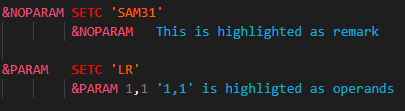
\includegraphics[width=10cm]{img/highligting}
	\caption{An example of highlighting.}
\end{figure}

\subsection{Autocomplete}
Autocomplete is enabled for the instruction field. While typing, a list of instructions starting with the typed characters displays. Selecting an instruction from the list completes it and inserts the default operands. Variables and sequence symbols are also filled with a value from their scope.

\begin{figure}[H]
	\centering
	\animategraphics[autoplay,loop,width=\linewidth]{12}{img/autocomplete/autocomplete-}{0}{126}
	\caption{\href{https://github.com/eclipse/che-che4z-lsp-for-hlasm/blob/master/readme\_res/autocomplete.gif}{Autocomplete usage example.}}
\end{figure}

\subsection{Go To Definition and Find All References}
The extension adds the functionality of \TT{go to definition} and \TT{find all references}. Use the \TT{go to definition} functionality to show definitions of variable symbols, ordinary symbols and macros, or open COPY files directly. Use the \TT{find all references} functionality to show all places where a symbol is used.

\begin{figure}[H]
	\centering
	\animategraphics[autoplay,loop,width=\linewidth]{12}{img/go_to_def/go_to_def-}{0}{90}
	\caption{\href{https://github.com/eclipse/che-che4z-lsp-for-hlasm/blob/master/readme\_res/go\_to\_def.gif}{Go To Definition usage example.}}
\end{figure}

\subsection{Macro Tracer}
The macro tracer functionality allows you to track the process of assembling HLASM code. It lets you see step-by-step how macros are expanded and displays values of variable symbols at different points during the assembly process. You can also set breakpoints in problematic sections of your conditional assembly code. 

The macro tracer is not a debugger. It cannot debug running executables, only track the compilation process.

\subsubsection{Configuring the Macro Tracer}

\begin{enumerate}
	\item Open your workspace.
	\item In the left sidebar, click the bug icon to open the debugging panel (Ctrl + Shift + D).
	\item Click create a launch.json file. A \TT{select environment} prompt displays.
	\item Enter \textbf{HLASM Macro tracer}. Your workspace is now configured for macro tracing.
\end{enumerate}

\subsubsection{Using the Macro Tracer}

To run the macro tracer, open the file that you want to trace. Then press \textbf{F5} to open the debugging panel and start the debugging session.

When the tracer stops at a macro or COPY instruction, you can select \textbf{step into} to open the macro or COPY file, or \textbf{step over} to skip to the next line.

Breakpoints can be set before or during the debugging session.

\begin{figure}[H]
	\centering
	\animategraphics[autoplay,loop,width=\linewidth]{12}{img/tracer/tracer-}{0}{398}
	\caption{\href{https://github.com/eclipse/che-che4z-lsp-for-hlasm/blob/master/readme\_res/tracer.gif}{Macro Tracer usage example.}}
\end{figure}

\end{document}
